% Created 2016-03-31 Thu 09:24
\documentclass[10pt,t,a4paper]{beamer}
\usepackage[utf8]{inputenc}
\usepackage[T1]{fontenc}
\usepackage{fixltx2e}
\usepackage{graphicx}
\usepackage{longtable}
\usepackage{float}
\usepackage{wrapfig}
\usepackage{rotating}
\usepackage[normalem]{ulem}
\usepackage{amsmath}
\usepackage{textcomp}
\usepackage{marvosym}
\usepackage{wasysym}
\usepackage{amssymb}
\usepackage{hyperref}
\tolerance=1000
\usetheme{BTH_msv}
\author{Mikael Svahnberg\thanks{Mikael.Svahnberg@bth.se}}
\date{2016-03-22}
\title{Modelling Behaviour \\\\ \texttt{PA14[13]5}}
\hypersetup{
  pdfkeywords={},
  pdfsubject={},
  pdfcreator={Emacs 25.1.50.1 (Org mode 8.2.10)}}
\begin{document}

\maketitle

\section{Contracts}
\label{sec-1}
\begin{frame}[label=sec-1-1]{Contracts}
\end{frame}
\begin{frame}[label=sec-1-2]{Summary}
\begin{itemize}
\item Black Box Description
\begin{itemize}
\item Use Cases
\item System Sequence Diagrams
\end{itemize}
\item White Box (first steps)
\begin{itemize}
\item Contracts
\end{itemize}
\end{itemize}
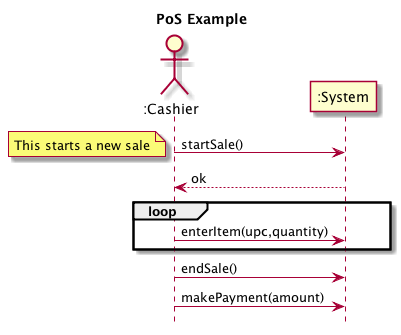
\includegraphics[height=4cm]{./FSystemSequenceDiagramExample.png}
\end{frame}
\begin{frame}[label=sec-1-3]{Stage-and-Curtain model}
\begin{itemize}
\item Visible: Current state

\emph{close curtains}

<things happen>

\emph{open curtains}

\item Visible: new state

The changes between current and new state are described in a \emph{Contract}
\end{itemize}
\end{frame}
\begin{frame}[label=sec-1-4]{State / System State}
\begin{itemize}
\item Concepts (Instances of)
\item Attributes (Values of)
\item Associations (Links between instances)
\end{itemize}
\end{frame}
\begin{frame}[label=sec-1-5]{Basic Contract Format}
\begin{itemize}
\item Name
\item Responsibles
\item Pre-conditions
\item Post-conditions
\end{itemize}
\end{frame}
\begin{frame}[label=sec-1-6]{Example}
\begin{itemize}
\item Name: \emph{EnterItem(barcode, quantity)}
\item Responsibilities: \emph{Record sale of an item and add it to the sale. Display item description and price.}
\item Preconditions: \emph{Sale is started}
\item Postconditions:
\begin{itemize}
\item \uline{:SalesItem} corresponding to product barcode was created.
\item \uline{:SalesItem} was associated with the current \uline{:Sale}
\item \uline{:SalesItem.quantity} was set to \emph{quantity}
\end{itemize}
\end{itemize}

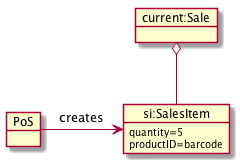
\includegraphics[height=3.5cm]{FContractExample.png}
\end{frame}
\begin{frame}[fragile,label=sec-1-7]{Preconditions}
 \begin{itemize}
\item Assumptions of the state of the system before operation begins
\item Not tested in the operation
\begin{itemize}
\item Ensured by the caller (!) \footnote{Defensive Programming says the exact opposite: if it is a precondition, then \verb~assert~ them so that you can fail early.}
\end{itemize}
\end{itemize}
\end{frame}
\begin{frame}[label=sec-1-8]{Postconditions}
Nature of postconditions:
\begin{itemize}
\item Declarative statements
\item Not ordered
\item Not actions performed: only state changes
\end{itemize}

Postcondition categories:     
\begin{itemize}
\item create or delete an instance
\item modification of an attribute
\item create or delete an association
\end{itemize}
\end{frame}
\begin{frame}[label=sec-1-9]{Extended Contract Format}
\begin{itemize}
\item Name: \emph{EnterItem(barcode, quantity)}
\item Responsibilities: \emph{Record sale of an item and add it to the sale. Display item description and price.}
\item Type: \emph{System}
\item Cross-References: \emph{Use case Buy Items, Requirements X, Y, Z}
\item Notes: \emph{Monitor speed of database query}
\item Exceptions: \emph{If barcode is invalid then indicate error}
\item Output: \emph{None}
\item Preconditions: \emph{Sale is started}
\item Postconditions:
\begin{itemize}
\item \uline{:SalesItem} corresponding to product barcode was created.
\item \uline{:SalesItem} was associated with the current \uline{:Sale}
\item \uline{:SalesItem.quantity} was set to \emph{quantity}
\end{itemize}
\end{itemize}
\end{frame}
% Emacs 25.1.50.1 (Org mode 8.2.10)
\end{document}